\chapter{Pendahuluan}

Bab Pendahuluan secara umum menceritakan landasan kerja dan arah kerja penulis tugas akhir, yang berfungsi untuk mengantar pembaca dalam memahami dan menganalisis laporan tugas akhir secara keseluruhan. Bab ini terdiri dari latar belakang, rumusan masalah, tujuan, batasan masalah, metodologi, dan jadwal pelaksanaan tugas akhir.

\section{Latar Belakang}
\label{sec:latarbelakang}

Teknologi dan internet adalah kebutuhan yang penting dalam kehidupan manusia di abad ke-21 ini. Salah satu bentuk teknologi modern paling berguna yang mudah diakses manusia adalah \emph{smartphone}, di mana akses internet sudah termasuk ke dalamnya. Berdasarkan penelitian yang dikumpulkan oleh \textcite{turner2022howmanysmartphones} pada bankmycell.com, pada tahun 2021 terdapat 6.37 miliar pengguna \emph{smartphone} di dunia atau sekitar 80.68\% dari populasi dunia, di antaranya 160.23 juta adalah penduduk Indonesia.

Banyak pekerjaan manusia yang dapat dilakukan dengan menggunakan berbagai jenis aplikasi yang dapat ditemukan dalam sebuah \emph{smartphone}. Menurut penelitian yang dilakukan oleh BusinessofApps, jumlah aplikasi pada iOS App Store ketika pertama kali diluncurkan pada tahun 2008 adalah 500, pada bulan November tahun 2021 angka tersebut melonjak menjadi 1.85 juta aplikasi. Pengguna Android memiliki lebih banyak pilihan dengan total 2.56 juta aplikasi di Google Play Store. Dengan banyaknya aplikasi tersebut, pada tahun 2020 pengguna \emph{smartphone} telah mengunduh aplikasi sebanyak 142.9 miliar kali, di antaranya 56.1 miliar unduhan adalah untuk aplikasi permainan \emph{mobile}.

Teknologi informasi yang semakin berkembang dapat meningkatkan kesejahteraaan digital, atau digital wellbeing, dari pengguna teknologi tersebut, beberapa caranya adalah meningkatkan koneksi sosial, mendukung kesehatan mental, dan mendukung kebiasaan sehat dengan fleksibilitas dalam praktik kerja. Namun teknologi informasi juga dapat menimbulkan akibat buruk yang memunculkan pola penggunaan teknologi yang tidak sehat. Beberapa contoh dampak buruk yang dimunculkan adalah mudahnya seseorang untuk kehilangan fokus, perasaan \emph{fear of missing out} (FoMO), serta kecanduan digital. Sifat-sifat buruk tersebut dapat lebih sering muncul ketika waktu yang dihabiskan pada dunia maya tidak diimbangi dengan waktu di dunia nyata. \parencite{ALMOURAD2021101778}

Pengaruh buruk seperti yang telah disebutkan di atas serta perilaku adiksi pada smartphone telah memunculkan perhatian bagi peneliti di bidang \textit{Human Computer Interaction} (HCI) untuk melakukan studi terhadap kesengajaan untuk tidak menggunakan teknologi. Pada saat ini, terdapat banyak perangkat lunak pada \textit{smartphone} yang bertujuan untuk mengubah perilaku penggunanya, di antaranya adalah Google. \parencite{Roffarello2019} Untuk membantu penggunanya, Google memiliki aplikasi Digital Wellbeing agar pengguna dapat memanfaatkan teknologi untuk meningkatkan kualitas kehidupannya melainkan menjadi distraksi. Pada websitenya tentang Digital Wellbeing, \textcite{google2019digitalwellbeing} mengatakan: "We’re committed to giving everyone the tools they need to develop their own sense of digital wellbeing. So that life, not the technology in it, stays front and center." 


Salah satu fitur yang terdapat pada aplikasi Digital Wellbeing adalah Focus Mode, sebuah fitur yang dapat membantu mengurangi distraksi dari \emph{smartphone} berbasis Android dengan cara memblokir sementara aplikasi yang dinilai sebagai distraksi. Focus Mode juga akan mendiamkan notifikasi yang masuk hingga waktu yang ditentukan. Waktu yang diterapkan untuk Focus Mode dapat diatur jadwalnya oleh pengguna. \parencite{android2019digitalwellbeing} Selama Focus Mode aktif, akan terdapat sebuah menu pada bagian notifikasi \emph{smartphone} dengan 2 buah fitur. Fitur "Take a break" yang berbentuk tombol ini dapat memberikan pengguna kembali akses untuk aplikasi yang diblok dengan pilihan waktu 5 menit, 15 menit, atau 30 menit. Tombol ini dapat digunakan jika pengguna ingin beristirahat dan menggunakan aplikasi yang diblok. Fitur "Turn off for now" yang juga berbentuk tombol dapat digunakan untuk memberhentikan Focus Mode hanya untuk hari tersebut. Tombol ini dapat digunakan jika pengguna merasa tugas yang perlu difokuskannya sudah selesai dan ingin menggunakan aplikasi yang diblok untuk sisa harinya. Masalah yang ditemukan dari Focus Mode terletak pada kedua fitur ini. Walau memerlukan interaksi lebih untuk "beristirahat", terdapat kemungkinan bagi pengguna untuk terus menerus mengakses aplikasi, dengan mengambil istirahat setiap beberapa menit sekali. Selain itu, fitur "Turn off for now" dapat disalahgunakan untuk menghindari Focus Mode secara keseluruhan.

\section{Rumusan Masalah}

Masalah utama dari sejumlah aplikasi yang ada dalam \emph{smartphone} adalah banyaknya distraksi dari aplikasi-aplikasi favorit yang dapat memperlambat kinerja pengguna. Distraksi-distraksi tersebut perlu diblok guna meningkatkan efektifitas pekerjaan seseorang. Fitur Focus Mode yang termasuk sebagai bagian dari aplikasi Digital Wellbeing milik Google dapat membantu untuk memblokir aplikasi, namun masih memiliki beberapa kekurangan dari desain interaksinya, seperti mudahnya pengguna dalam menghindari blok dengan menekan tombol "Take a break" berkali-kali atau cukup menekan tombol "Turn off for now" untuk mematikan Focus Mode pada hari tersebut. Maka dari itu, dapat disimpulkan rumusan masalah yang akan didalami adalah sebagai berikut.

\begin{enumerate}
  \item Apa \emph{usability} dan \emph{user experience goals} yang tepat untuk membangun rancangan desain interaksi aplikasi pencegah distraksi?
  \item Bagaimana prototipe aplikasi pencegah distraksi dengan desain interaksi menggunakan pendekatan \emph{user-centered design}?
\end{enumerate}

\section{Tujuan}

Berdasarkan latar belakang dan rumusan masalah di atas, tujuan dari Tugas Akhir ini adalah untuk membuat sebuah prototipe aplikasi pencegah distraksi. Prototipe aplikasi tersebut memiliki desain interaksi yang dapat menyelesaikan masalah-masalah desain interaksi yang ditemukan pada alat Digital Wellbeing milik Google, terutama pada fitur Focus Mode.

\section{Batasan Masalah}

Batasan masalah untuk implementasi solusi Tugas Akhir ini adalah sebagai berikut.
\begin{enumerate}
  \item Prototipe aplikasi akan diimplementasi hanya untuk \textit{platform} Android.
  \item Pengujian akan difokuskan di kalangan pengguna \textit{smartphone} Android yang menggunakan alat Digital Wellbeing.
\end{enumerate}

\section{Metodologi}
\label{sec:metodologi}

Metodologi yang akan digunakan dalam Tugas Akhir adalah pendekatan \textit{user-centered design} (UCD). Metodologi UCD mengikuti standar alur kerja dari ISO (\textit{International Organization for Standardization}) 9241-210:2010 yang diilustrasikan pada Gambar \ref{fig:diagram_iso1}. Beberapa tahap dari UCD akan dilakukan secara iteratif, dengan penjelasan sebagai berikut: 


\begin{figure}[h]
  \centering
  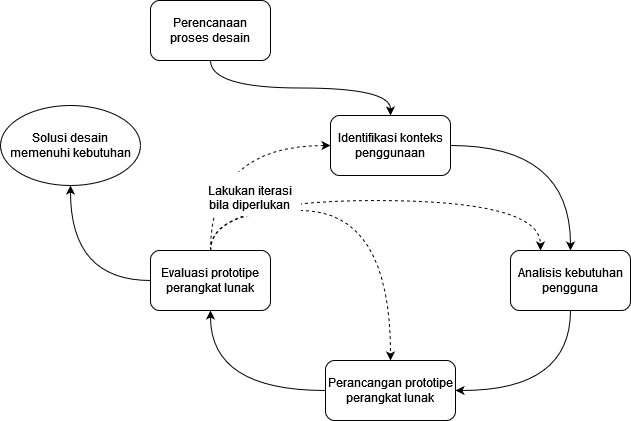
\includegraphics[width=0.9\textwidth]{chapter-1-method.png}
  \caption{Diagram alur pengerjaan \textit{User-Centered Design} (ISO 9241-210, 2010)}
  \label{fig:diagram_iso1}
\end{figure}

\begin{enumerate}
  \item Perencanaan proses desain
  \subitem Proses UCD diawali dengan tahap persiapan, yaitu proses perancangan terhadap lingkup aplikasi yang dibuat serta perencanaan untuk pengambilan data. Lingkup dari aplikasi termasuk jenis antarmuka dan \textit{platform} yang dipilih untuk implementasi, lingkup fungsionalitas aplikasi, serta target pengguna aplikasi. Sedangkan perencanaan pengambilan data dilakukan dengan cara survei dan wawancara.

  \item Identifikasi konteks penggunaan
  \subitem Pada tahap ini dilakukan pengumpulan data pengguna melalui survei dan wawancara sesuai dengan kebutuhan. Data yang didapatkan akan dianalisis untuk mengungkapkan permasalahan, kebutuhan, dan tujuan pengguna. Berdasarkan data riset tersebut akan dibentuk persona serta skenario penggunaan aplikasi, yang kemudian akan dianalisis untuk mendapatkan kebutuhan perangkat lunak.
   
  \item Analisis kebutuhan perangkat lunak
  \subitem Tahap ini terdiri dari analisis fitur perangkat lunak, analisis \textit{user experience goals}, dan analisis \textit{usability goals}. Fitur-fitur yang terkumpul akan menjadi bahan implementasi pada tahap selanjutnya.
  
  \item Perancangan prototipe perangkat lunak
  \subitem Rancangan kebutuhan perangkat lunak yang sudah dikumpulkan pada tahap sebelumnya akan kemudian diimplementasikan, mulai dari \textit{low-fidelity prototype}, \textit{high-fidelity prototype}, kemudian menjadi sebuah prototipe aplikasi. Hal ini dilakukan untuk meningkatkan kualitas data yang didapatkan selama tahap evaluasi karena keperluan prototipe aplikasi untuk digunakan sepanjang hari dalam jangka waktu lama. Proses ini dilakukan secara iteratif bersamaan dengan tahap evaluasi.
  
  \item Evaluasi prototipe perangkat lunak
  \subitem Tahap evaluasi dilakukan untuk menguji solusi desain yang telah dirancang, apakah solusi telah memenuhi kebutuhan pengguna dan \textit{user experience goals} serta \textit{usability goals} yang ditargetkan. Hasil evaluasi akan menentukan apakah desain yang diuji perlu diperbaiki dalam proses iterasi.
  
\end{enumerate}

% desecara garis besar akan terdiri dari perencanaan, analisis ruang lingkup, analisis kebutuhan pengguna, analisis desain solusi, dan pengujian desain solusi. Sebagai tambahan, aplikasi juga akan diimplementasi dalam tahap pengujian agar mendapatkan data untuk membuktikan efektifitas dari desain interaksinya.

\section{Jadwal Pelaksanaan Tugas Akhir}

Jadwal pengerjaan dari Laporan Tugas Akhir ini adalah sebagai berikut.

\begin{figure}[h]
  \centering
  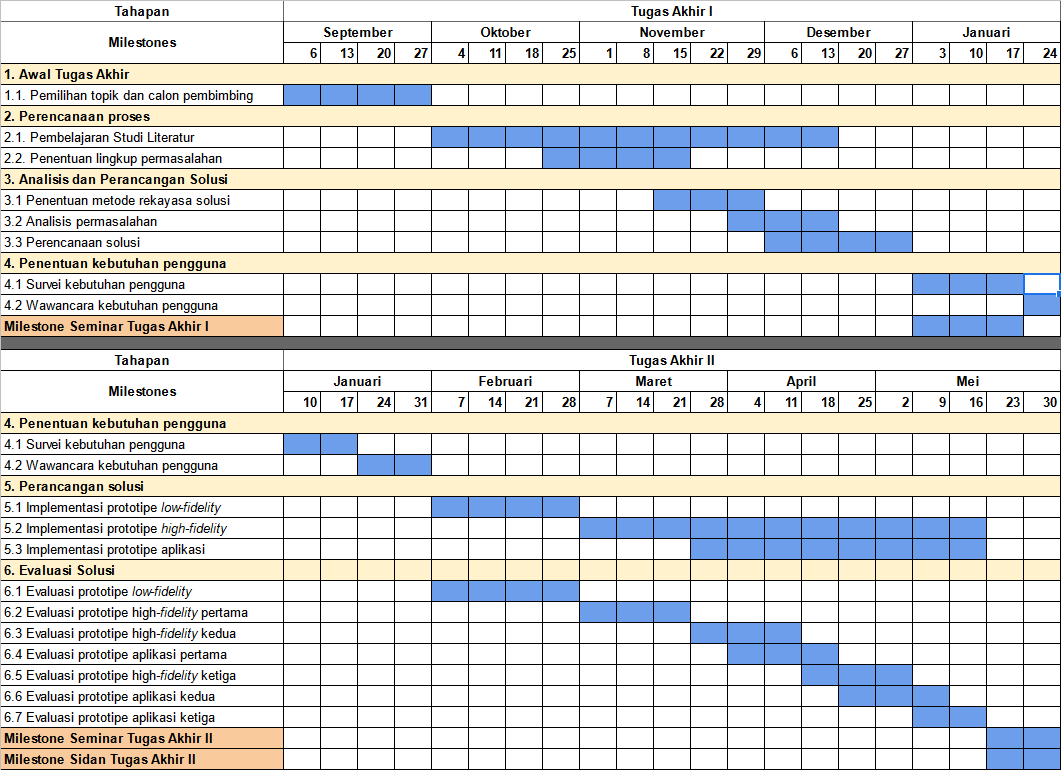
\includegraphics[width=\textwidth]{chapter-1-jadwal-TA.png}
  \caption{Jadwal Pelaksanaan Tugas Akhir}
\end{figure}
